\documentclass[a4paper,11pt]{article}

\usepackage{color}
\usepackage{graphicx}
\usepackage[margin=20mm]{geometry} % minimum this should be is 15mm
\usepackage{wrapfig}

% Highlighting macros
\newcommand{\red}[1]{{\textcolor{red}{#1}}}
\newcommand{\green}[1]{{\textcolor{green}{#1}}}
\newcommand{\blue}[1]{{\textcolor{blue}{#1}}}
\newcommand{\changed}[2][{}]{\red{\sout{#1}}\blue{#2}}
\newcommand{\todo}[1]{{\bf ***\red{#1}***}}
\newcommand{\comment}[1]{\blue{#1}} %comments

\parindent=0pt
\pagestyle{empty}

\begin{document}

\section*{First Light And Reionisation Epoch Simulations (FLARES)}

We propose a suite of simulations of galaxy formation at very high redshift
($z>5$) with the aim of: making predictions for observations by JWST, Euclid, and
other upcoming facilities; elucidating the contribution of the first galaxies to
reionization.  We will use resimulations of regions chosen at $z=5$ to (i) obtain
a large sample of massive, high-luminosity galaxies; (ii) explore a wide range
of environments.

\todo{Stephen to provide some observational motivation.}

(i) To obtain a large sample of high-redshift galaxies, we need to resimulate
overdense regions in the early universe.  We use as our background simulation
the same 3.2 Gpc box previously used for the Bahamas (Bahe etal 2017) and
C-EAGLE (Barnes etal 2017) projects.  As demonstrated by Lovell etal (2018) and
others, there is a large mismatch between overdensities at z=0 (as used by the
above projects) and those at z=5; whereas at z=5 and above, the fluctuations are
linear on the scales that we resimulate: for that reason, we resimulate
spherical regions of high overdensity identified at that redshift.

\begin{wrapfigure}{r}{0.5\textwidth}
  \centering
  \vspace*{-0.9cm}
  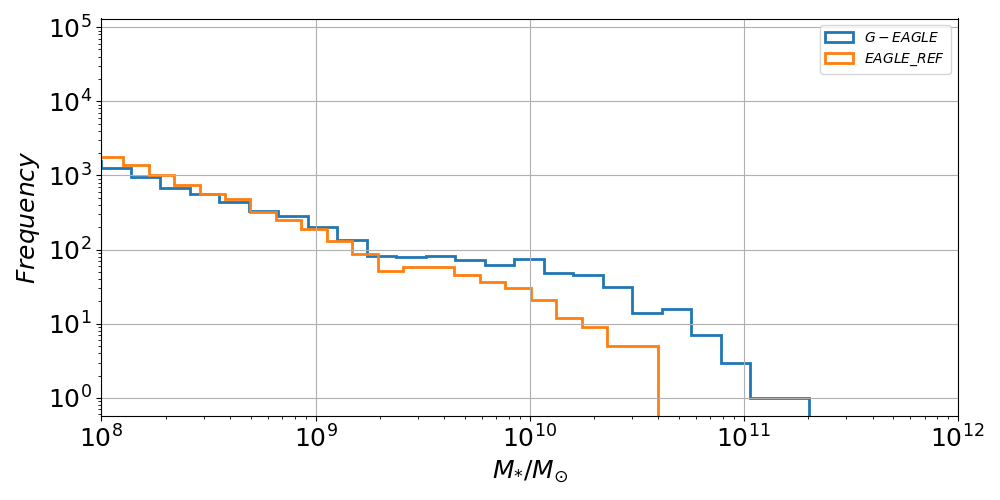
\includegraphics[width=0.48\textwidth]{FLARES_ngal.png}
  \caption{Number of galaxies in the EAGLE simulation (orange) and in test
    simulations (blue) at $z=5$, as described in the text.}
  \label{fig:FLARES_ngal}
\end{wrapfigure}

Figure~\ref{fig:FLARES_ngal} shows the combined results of 5 test simulations
(labelled G-EAGLE) that together comprise just five-eighths of the volume of one
of our proposed resimulations, as compared to the number of galaxies in the
EAGLE reference volume (Furlong etal 2015).  This shows two things: firstly that
resimulation technique is extremely efficient in probing the sites of galaxy
formation at high redshift; and secondly that it probes the highest mass
galaxies that are simply not present in smaller boxes which fail to sample the
long-wavelength modes of the power spectrum.

\todo{Plot and discussion about sampling of rare objects.}

(ii) \todo{Discussion of cosmic variance.}

{\bf Technical details:}This proposal will use the well-tested and highly
successful galaxy simulation software suite used for the EAGLE simulation
(Schaye etal 2015) and in cluster resimulations (Bahe etal 2017, Barnes etal
2017).  We will use the P-Gadget3 EAGLE code with the AGNdT9 normalisation for
AGN feedback.  Outputs will be analysed using SUBFIND to identify halos,
sub-halos and galaxies.  Test runs have been performed on which the figures used
above and in the technical case are based.

\todo{Summarise numbers that I gave to Adrian}

\end{document}
